%===============================================================================
\section{Rationale For Global Pairing through Optimal Transport}
\label{app:ot}
%===============================================================================

As discussed in \cref{sec:methods}, random pairing of control and perturbed cells leads to mean collapse. Here, we detail the mechanism behind this phenomenon and the mathematical formulation of our \gls{ot} solution.

\subsection{Mechanism of Mean Collapse}

For a given interventional sample (e.g., cell $i$, in which gene $A$ was perturbed), a randomly selected observational sample (e.g., cell $j$) from the batch is highly unlikely to be an appropriate counterfactual. 
The biological state of cell $j$ may differ substantially from that of cell $i$ prior to the perturbation.
Consequently, the model must learn a transformation from an often noisy and biologically irrelevant initial state. 
Across thousands of training iterations, a single interventional sample is paired with hundreds of different random controls. Each pairing provides a distinct and noisy gradient signal. 
The optimiser seeks to minimise the loss on average across these inconsistent pairings and converges on a simple solution: predicting the mean of the target distribution. The random noise from the poor counterfactuals averages to zero, leaving only the central tendency as a stable learning signal. Ultimately, the objective function effectively becomes an expectation over these random pairings. The model learns that the most reliable strategy to achieve a low expected loss is to ignore the specifics of the randomly chosen input and produce an average output. The optimisation landscape is thereby smoothed in a manner that makes the `mean prediction' an attractive local minimum.

\begin{figure}[tb]
    \centering
    \begin{subfigure}{0.45\linewidth}
        \centering
        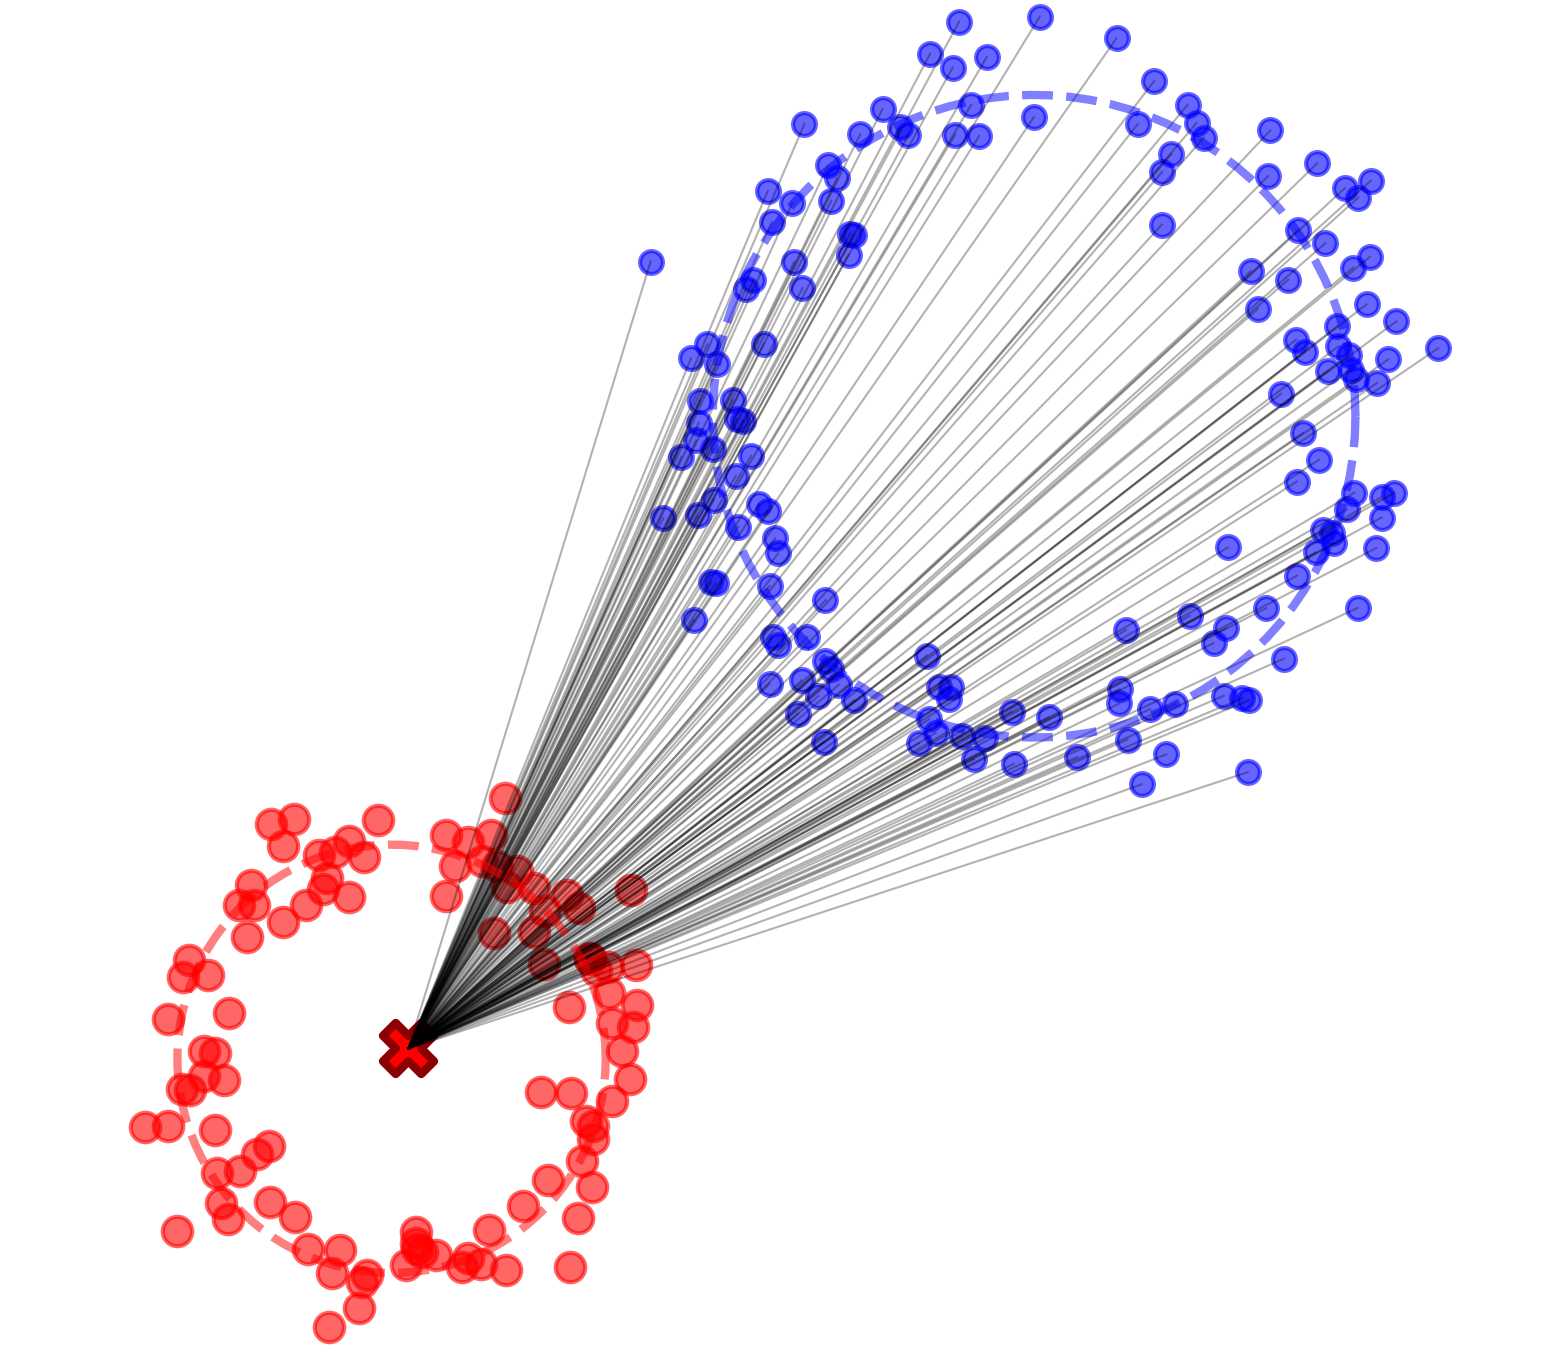
\includegraphics[width=\linewidth]{gfx/OT.png}
        \caption{Random pairing}
        \label{fig:app:ot_comparison_a}
    \end{subfigure}
    \hfill
    \begin{subfigure}{0.45\linewidth}
        \centering
        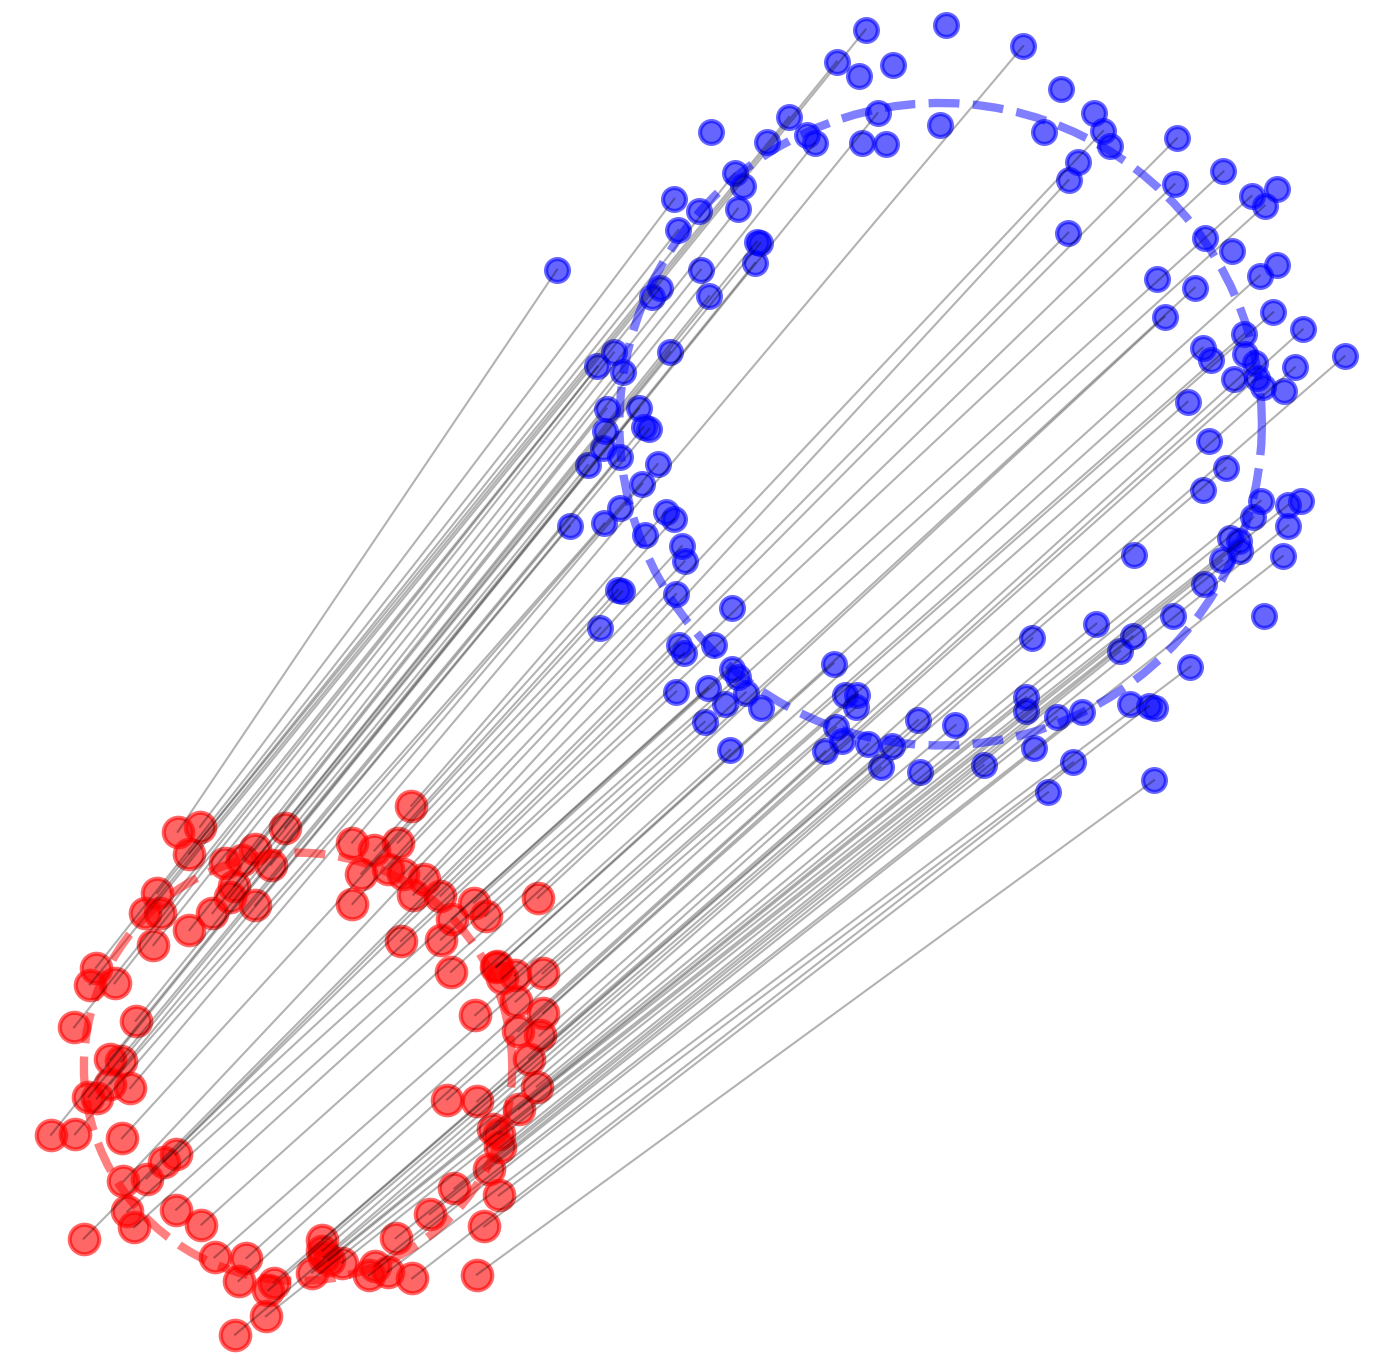
\includegraphics[width=\linewidth]{gfx/ot_comparison.png}
        \caption{Optimal Transport}
        \label{fig:app:ot_comparison_b}
    \end{subfigure}
    \caption{
        \textbf{Comparison of random pairing vs. Optimal Transport.}
        (a) Random pairing collapses the source distribution towards the target mean (mean collapse).
        (b) Optimal Transport pairing preserves the underlying population structure and biological heterogeneity.
    }
    \label{fig:app:ot_comparison}
\end{figure}

Rather than creating noisy one-to-one random pairs, \glsentryshort{ot} considers the entire population of observational and interventional latents. 
It computes an optimal flow of probability mass from the observational to the interventional distribution. This flow represents the most efficient method of morphing one entire point cloud into the other. The flow implicitly creates meaningful pairings.
Each interventional sample is matched with the observational sample(s) that are closest in gene expression space, providing the best possible counterfactuals within the given populations.
\revised{The theoretical properties of \glsentryshort{ot} ensure that it robustly preserves the inherent heterogeneous subpopulation structures by minimizing the ground movement cost, a feature critical for reliable counterfactual prediction.}

\subsection{Formal Derivation of Mean Collapse}
\revised{
We formally demonstrate why the random pairing strategy used in many current approaches fails to capture heterogeneous cellular responses.
Let $\variables \in \observsupport$ represent the control (source) cell and $\variables' \in \interventionaldist$ represent the perturbed (target) cell under intervention $p$. A generative model $\practicalencoder(\variables, p)$ aims to minimize the expected reconstruction error:
\begin{equation}
    \mseloss(\theta) = \mathbb{E}_{\variables \sim \observsupport, \variables' \sim \interventionaldist} \left[ \| \variables' - \practicalencoder(\variables, p) \|^2 \right]
\end{equation}

By the principles of Minimum Mean Squared Error (MMSE) estimation, the optimal function $f^*(\variables, p)$ that minimizes this loss is the conditional expectation:

\begin{equation}
    f^*(\variables, p) = \mathbb{E}[\variables' \mid \variables, P=p]
\end{equation}
In the case of \textbf{random pairing}, the target cell $\variables'$ is selected independently of the input cell $\variables$ (i.e., $\variables' \perp \variables \mid P=p$). This conditional independence allows us to simplify the expectation:
\begin{equation}
    f^*(\variables, p) = \mathbb{E}[\variables' \mid P=p] = \bar{\variables}_p
\end{equation}
where $\bar{\variables}_p = \int \variables' p(\variables' \mid P=p) d\variables'$ is the population mean vector for all cells undergoing perturbation $p$. 

\textbf{Conclusion:} Under random pairing, the model's optimal mathematical strategy is to completely ignore the specific initial state $\variables$ and predict a constant mean response for the entire population. This results in a Jacobian $\nabla_{\variables} f \to 0$, effectively erasing any discoverable \textit{cell-specific treatment effects}. By using \gls{ot} to enforce a deterministic coupling where $I(\variables, \variables') > 0$, \glsentryshort{raptorgraph} ensures that the model preserves the biological trajectory of individual cells.
}

\subsection{Mathematical Formulation of Optimal Transport}
Let $\mu_s = \sum_{i=1}^n \frac{1}{n} \delta_{\zobs^{(i)}}$ and $\nu_t = \sum_{j=1}^m \frac{1}{m} \delta_{\zint^{(j)}}$ be the empirical measures of the source (control) and target (perturbed) latent distributions.
The Optimal Transport problem seeks a transport plan $\gamma \in \mathbb{R}_{+}^{n \times m}$ that minimizes the total cost:
\begin{equation}
    \min_{\gamma \in \Pi(\mu_s, \nu_t)} \langle \gamma, \mathbf{C} \rangle_F
\end{equation}
where $\mathbf{C}_{ij} = \| \zobs^{(i)} - \zint^{(j)} \|^2_2$ is the squared Euclidean cost matrix, and $\Pi(\mu_s, \nu_t)$ is the set of joint probability measures with marginals $\mu_s$ and $\nu_t$.
The resulting optimal plan $\gamma^*$ provides a probabilistic coupling. To obtain a deterministic mapping for training, we use the barycentric projection map, ensuring each control cell is paired with its optimal counterfactual representation in the perturbed domain.

% [ADDITION: Addressing Reviewer yvAn] Added technical comparison between Hungarian matching 
% and Sinkhorn OT to justify why "soft" probabilistic coupling is more stable for scRNA-seq.
\subsection{\revised{Alternative Pairing Strategies}}
\label{app:ot:alternatives}

\revised{
To contextualize the performance of Sinkhorn \gls{ot}, we compare it against two common structured pairing alternatives:
\begin{itemize}
    \item \textbf{Nearest Neighbor (NN) Matching:} For each perturbed cell $\variables' \in \mathcal{Y}_p$, we select the control cell $\variables \in \mathcal{X}$ that minimizes the Euclidean distance $\|\variables - \variables'\|_2$. This is a greedy, many-to-one mapping strategy. While computationally efficient, it often fails to preserve the global distribution of the control population, leading to redundant pairings and loss of heterogeneity.
    \item \textbf{Hungarian Matching (Linear Sum Assignment):} This approach solves the bipartite matching problem to find a strict one-to-one bijection between control and perturbed sets by minimizing the total assignment cost $\sum_{i} \mathbf{C}_{i, \sigma(i)}$. We implement this using the Kuhn-Munkres algorithm. While globally optimal in a discrete sense, the hard assignment is highly sensitive to outliers and sampling noise in \gls{scRNAseq} data, leading to the instability observed in our results.
\end{itemize}
}
